%!TEX root = ./thesis-main.tex
%-------------------------------------------------------------------------------
% 								BAB I
% 							LATAR BELAKANG
%-------------------------------------------------------------------------------

\chapter{LATAR BELAKANG}

\section{Latar Belakang Masalah}
Kota Palembang selalu berhias diri dikarenakan Kota Palembang dipercaya menjadi pusat penyelenggaraan kegiatan bertaraf nasional maupun internasional. Banyak kegiatan yang sudah dilaksanakan di Kota Palembang antara lain \emph{SEA Games XXVI}, MTQ Internasional, Konferensi Negara Islam Ke-7, Kejuaraan Golf Internasional, Kejuaraan Musi TriBoatton (MTT), Kejuaraan Ski Air, Beach Volley se Asia Pacific, \emph{Asia Junior Swimming Competition} dan \emph{ASEAN Games} yang akan diadakan pada tahun 2018 mendatang. Untuk mendukung kegiatan-kegiatan tersebut maka berbagai sarana publik terus di bangun seperti Jembatan \emph{FlyOver}, dan yang terbaru adalah pembangunan \emph{Light Rail Transit (LRT)} untuk mendukung ASEAN Games yang akan datang. Kegiatan nasional dan internasional berdampak sangat positif terhadap perkembangan pembangunan Kota Palembang. \\

\begin{figure}[H]
  \centering
    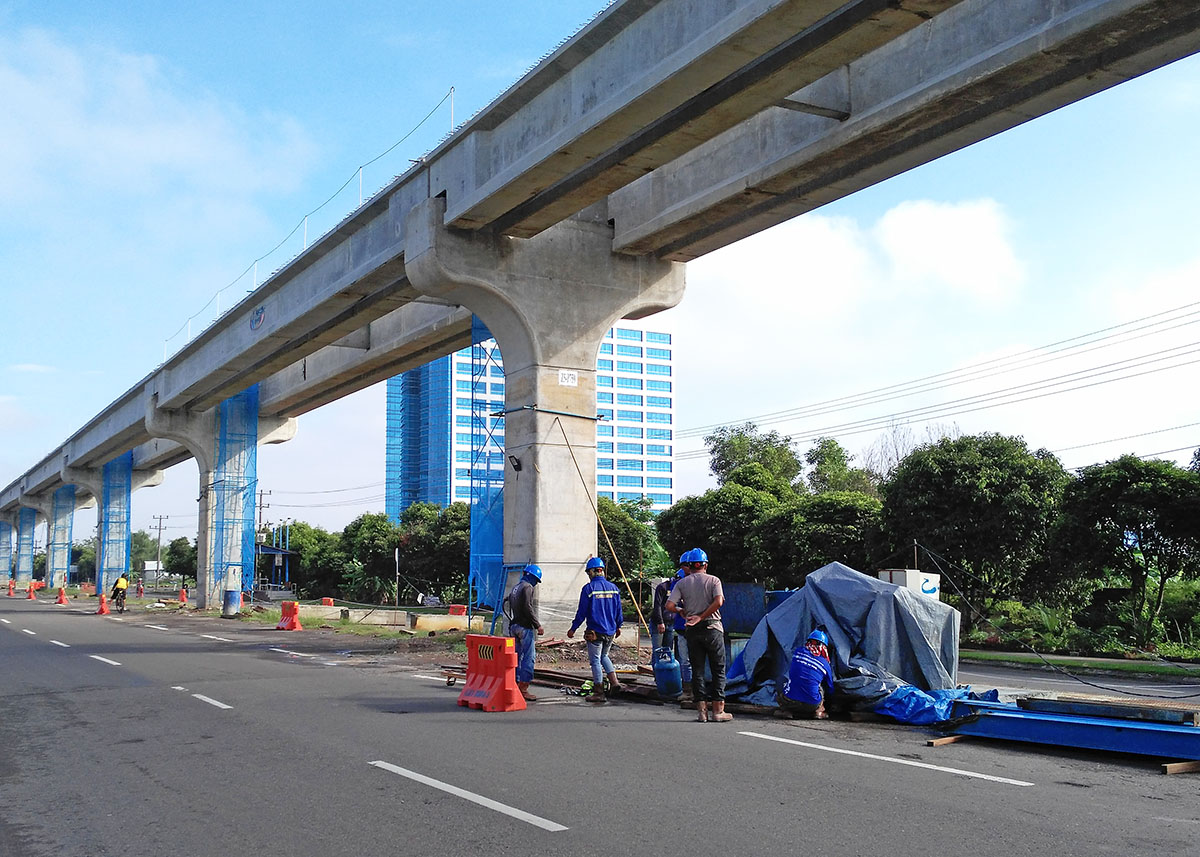
\includegraphics[scale=0.2]{gambar/lrt.jpg}
    \caption{Pembangunan LRT Palembang (Todes/bulletinmetropolis.com, 2017)}
    \label{fig:lrt}
\end{figure}

Selain dampak dari segi pembangunan kota dampak lain dari kegiatan tersebut adalah meningkatnya jumlah wisatawan yang berkunjung ke Kota Palembang sehingga turut meningkatkan kepariwisataan Kota Palembang. Statistik kunjungan kota Palembang ditunjukkan ditunjukkan pada Gambar \ref{fig:bps}.\\

\begin{figure}[H]
  \centering
    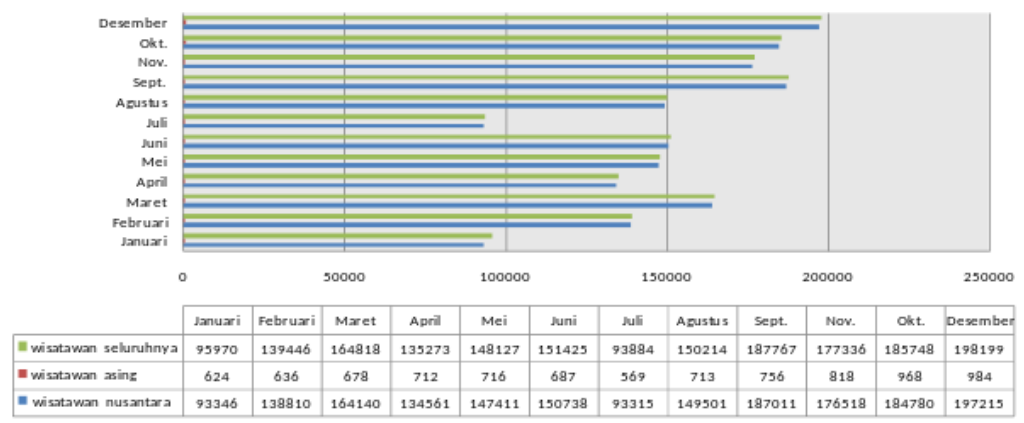
\includegraphics[scale=0.41]{gambar/bps.png}
    \caption{Statistik kunjungan wisata ke Kota Palembang (BPS Kota Palembang, 2014}
    \label{fig:bps}
\end{figure}

Berdasarkan Gambar \ref{fig:bps} terlihat bahwa terjadi peningkatan jumlah wisatawan yang masuk ke Palembang. Wisatawan lokal dan manca negara banyak berdatangan untuk menghadiri berbagai kegiatan yang diadakan di Palembang, hal ini ikut memicu banyaknya pemesanan hotel, penggunaan fasilitas umum berupa hotel, supermarket, pasar, halte bus, mesin ATM, rumah sakit, restoran atau rumah makan, tempat hiburan, tempat wisata dan lain sebagainya untuk mendukung kegiatan para wisatawan selama berada dan tinggal di Palembang.\

Untuk membantu mobilitas wisatawan yang datang ke Palembang maka dibutuhkan sebuah media yang dapat membantu mereka mendapatkan info mengenai event-event, sarana transportasi, serta fasilitas publik untuk mengakomodasi mereka selama event-event tersebut berlangsung. Informasi tersebut saat ini belum tersedia secara komprehensif bagi para wisatawan. Website-website resmi dari pemerintah hanya menampilkan informasi kegiatan serta berita-berita lain tentang Palembang, tetapi belum ada informasi yang cukup tentang fasilitas publik kota Palembang.\ 
Kota Palembang telah memiliki portal informasi resmi pada alamat http://www.palembang.go.id/. Terdapat informasi-informasi publik untuk berbagai bidang seperti kesehatan, pendidikan, pariwisata, dll.\
\begin{figure}[H]
  \centering
    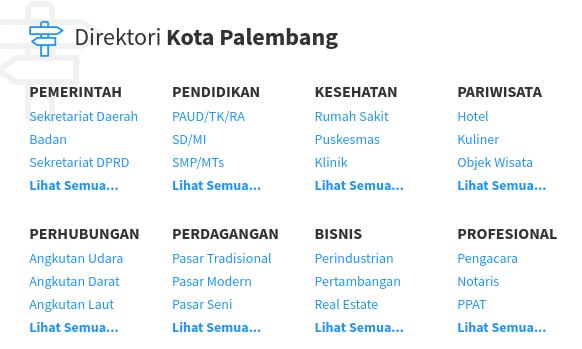
\includegraphics[scale=0.7]{gambar/palembanggoid.png}
    \caption{Potongan Website Direktori Kota Palembang (Pemerintah Kota Palembang, 2017)}
    \label{fig:plgportal}
\end{figure}
Pada gambar \ref{fig:plgportal} terdapat informasi-informasi mengenai kota Palembang yang terbagi kedalam direktori-direktori. Setiap informasi dipisahkan oleh \emph{link-link}  yang berbeda. Pengguna harus melakukan navigasi berulang kali untuk mendapatkan informasi-informasi yang berbeda tersebut. Cohen dalam Booth (2015) menyatakan bahwa sistem navigasi seperti ini (\emph{menu-based systems}) dapat digunakan untuk mencari informasi dengan mudah, tetapi kemampuan pencariannya sudah ditentukan sebelumnya dan tidak fleksibel.\

Oleh karena itu, untuk mengatasi keterbatasan tersebut dapat digunakan bahasa alami. Kauffman dalam Booth (2015) menyatakan bahwa bahasa alami lebih baik dalam menyatakan pertanyaan atau perintah, terlebih yang membutuhkan informasi negasi, jumlah dan informasi temporal. Bahasa alami juga mengurangi waktu penyelesaian suatu tugas.\

Penggunaan pencarian berbasis semantik pada sistem yang akan diajukan diharapkan dapat memberikan hasil yang lebih sesuai dengan konteks yang diinginkan pengguna. Penelitian tentang pencarian berbasis semantik pernah dilakukan oleh Admojo (2015), pada penelitian tersebut digunakan input dari query bahasa alami yang seterusnya akan ditulis \emph{NLP (Natural Language Processing)}. Domain Ontologi yang digunakan pada penelitian tersebut adalah \emph{linguistic} dan \emph{mountaineering}. Hasil penelitian mampu memahami input bahasa alami secara sintaksis dan secara semantik.\

Booth (2015) dalam penelitiannya mengembangkan sebuah bahasa query untuk perencanaan perjalanan yang diberi nama \emph{TRANQUYL}. Selanjutnya mereka juga mengembangkan software bernama \emph{NL2TRNQUYL} yang menerjemahkan input bahasa inggris menjadi \emph{query} yang dimengerti oleh \emph{TRANQUYL}. Sistem tersebut mampu mengerti \emph{request} dari user baik itu berupa kalimat utuh ataupun hanya potongan kalimat saja.\

Berdasarkan penelitian-penelitian tersebut diusulkan sebuah sistem dimana pengguna bisa memberikan input berupa \emph{query NLP} dalam bahasa Indonesia dan mendapatkan hasil sesuai dengan yang diharapkan.


\section{Rumusan Masalah}
Rumusan masalah dalam penelitian ini adalah bagaimana menyediakan informasi \emph{event} dan fasilitas publik Kota Palembang yang memadai bagi wisatawan  dengan input pengguna berupa bahasa alami.\


\section{Batasan Masalah}
Agar penelitian ini tetap fokus maka diberikan batasan-batasan sebagai berikut:
\begin{enumerate}
  \item Input bahasa yang digunakan menggunakan bahasa Indonesia
  \item Data fasilitas publik yang ditampilkan berupa Rumah Sakit, Tempat Ibadah, Tempat Wisata dan Tempat Makan
  \item Data koordinat fasilitas publik didapat dari layanan \emph{Foursquare} dan \emph{Google Map API}.
  \item Bahasa Pemrograman yang akan digunakan pada thesis ini adalah \emph{PHP} untuk \emph{Backend}, \emph{Javascript} pada bagian \emph{Frontend}. \emph{Database} menggunakan \emph{RDF Triple Store}, yang akan di akses menggunakan sebuah \emph{project Open Source} bernama \emph{Apache Jena Fuseki}.
  \item Sistem akan memberikan \emph{output} berupa \emph{JSON} yang dapat di konsumsi oleh \emph{client} lintas platform. 
\end{enumerate}


\section{Tujuan Penelitian}
Tujuan dari penelitian ini adalah menghasilkan piranti lunak yang memberikan solusi untuk permasalahan pencarian informasi kegiatan beserta fasilitas publik kota Palembang dengan menyusun ontologi untuk merepresentasikan basis pengetahuan berupa data fasilitas umum di Kota Palembang beserta rute transportasinya berdasarkan input \emph{NLP}.


\section{Manfaat Penelitian}
Manfaat dari penelitian ini adalah:
\begin{enumerate}
  \item Membantu wisatawan mendapatkan informasi publik fasilitas umum di Kota Palembang.
  \item Membantu wisatawan mendapatkan informasi kegiatan-kegiatan di Kota Palembang.
\end{enumerate}

\section{Sistematika Penulisan}
\noindent
\textbf{BAB I : PENDAHULUAN}

Pada bab ini dijelaskan latar belakang, rumusan masalah, batasan, tujuan, manfaat, dan sistematika penulisan.\\

\noindent
\textbf{BAB II : TINJAUAN PUSTAKA}

Pada bab ini diuraikan teori-teori dasar yang berkaitan dengan penelitian-penelitian yang telah dilakukan.\\

\noindent
\textbf{BAB III : LANDASAN TEORI}

Pada bab ini dijelaskan teori-teori dasar yang berkaitan dengan penelitian yang dilakukan dan akanmenjadi dasar dalam pemecahan masalah.\\

\noindent
\textbf{BAB IV : ANALISIS DAN RANCANGAN SISTEM}

Pada bab ini dijelaskan perancangan ontologi bahasa dan fasilitas publik Kota Palembang, proses pada setiap tahapan pada rancangan arsitektur penelitian serta perancangan antarmuka sistem.\\

\noindent
\textbf{BAB V : IMPLEMENTASI}

Bab ini berisikan pembuatan class, property, dan instance pada ontologi yang digunakan serta pembahasan proses yang terjadi dari input \emph{NLP} pengguna sampai ke hasil akhir yang dapat diproses oleh antarmuka sistem.\\

\noindent
\textbf{BAB V : HASIL DAN PEMBAHASAN}

Pada bab ini dijelaskan hasil penelitian dan pembahasannya.\\

\noindent
\textbf{BAB V : KESIMPULAN DAN SARAN}

Pada bab ini ditulis kesimpulan akhir dari penelitian dan saran untuk pengembangan penelitian selanjutnya.\\

% Baris ini digunakan untuk membantu dalam melakukan sitasi
% Karena diapit dengan comment, maka baris ini akan diabaikan
% oleh compiler LaTeX.
\begin{comment}
\bibliography{daftar-pustaka}
\end{comment}
